\documentclass{template}
\bibliographystyle{plainnat}

\usepackage{import}

\usepackage{microtype}

\usepackage{setspace}

\usepackage{amsmath}

\usepackage{amsfonts}

\usepackage{amssymb}
\usepackage{bbm}
\usepackage{graphicx}

\usepackage{hyperref}

\usepackage{breqn}

\usepackage{color}

\usepackage{listings}

% Set various options for exam package


% Set lesson name, etc.



\usepackage{enumitem}


% Set headers/footers to look nice





% Define commands related to marking up content

\newcommand{\source}[1]{}

\allowdisplaybreaks

% Define commands related to general mathematical style

%\renewcommand{\exp}[1]{e^{#1}}
\renewcommand{\exp}[1]{\text{exp}\left\{#1\right\}}

\newcommand{\beq}{\begin{equation}}

\newcommand{\eeq}{\end{equation}}

\newcommand{\bpart}{\begin{parts}}

\newcommand{\epart}{\end{parts}}

\newcommand{\bsol}{\begin{solution}}

\newcommand{\esol}{\end{solution}}

\newcommand{\for}{\text{\ for\ }}

\def\bal#1\eal{\begin{align*}#1\end{align*}}

\newcommand{\bmat}{\begin{pmatrix}}

\newcommand{\emat}{\end{pmatrix}}

\newcommand{\tab}{\hspace*{2em}}
\newcommand{\wrd}[1]{\hspace{-1in}\text{#1}}


  \newcommand{\intinf}{\int_{0}^{\infty}}
    \newcommand{\intinff}{\int_{-\infty}^{\infty}}
  \newcommand{\vertinf}{\vert_{0}^{\infty}}
\newcommand{\pois}{\text{Poisson}}
\newcommand{\bin}{\text{Bin}}
\newcommand{\pole}{\Big{|}}
\newcommand{\sumi}{\sum_{i=1}^n}
\newcommand{\sumj}{\sum_{j=1}^n}
\newcommand{\sumk}{\sum_{k=1}^n}

\newcommand{\prodi}{\prod_{i=1}^n}
\usepackage{afterpage}
\newcommand{\npdf}{\frac{1}{\sigma\sqrt{2\pi}}e^{-\frac{(x_i-\mu)^2}{2\sigma^2}}}
\newcommand{\parthe}[1]{\frac{\partial}{\partial #1}}
\newcommand\blankpage{%
    \null
    \thispagestyle{empty}%
    \addtocounter{page}{-1}%
    \newpage}
\newcommand{\var}[1]{\text{Var}\paren{#1}}
\newcommand{\skw}{\text{Skew}}
\newcommand{\kurt}{\text{Kurt}}
\newcommand{\corr}{\text{corr}}
\newcommand{\cov}{\text{Cov}}
\newcommand{\ind}{\mathbf{1}}
\newcommand{\N}{\mathcal{N}}
\newcommand{\B}{\mathcal{B}}
\renewcommand{\P}{\mathcal{P}}
\newcommand{\E}{\mathcal{E}}
\newcommand{\U}{\mathcal{U}}
\renewcommand{\L}{\mathcal{L}}
\newcommand{\bone}{\ind}
\newcommand{\J}{\mathcal{J}}
\newcommand{\R}{\mathbb{R}}
\newcommand{\I}{\mathbb{I}}
\newcommand{\indep}{\rotatebox[origin=c]{90}{$\models$}}
\newcommand{\myqed}{\text{\rule{3ex}{3ex}
\hspace{-.25in}
\textcolor{white}{$\mathcal{B}$}}}
\newcommand{\paren}[1]{\left(#1\right)}
\renewcommand{\brack}[1]{\left[#1\right]}
\usepackage{verbatim}
\newcommand{\abs}[1]{\left\vert #1 \right\vert}

\renewcommand{\exp}[1]{\text{exp}\left\{#1\right\}}
\newcommand{\mle}[1]{\hat{#1}_{MLE}}
\newcommand{\eps}{\varepsilon}
\newcommand{\st}{\text{ s.t. }}
\newcommand{\parder}[2]{\dfrac{\partial #1}{\partial #2}}
\newcommand{\aveX}{\overline{X}_n}
\makeatletter
\newcommand{\pushright}[1]{\ifmeasuring@#1\else\omit\hfill$\displaystyle#1$\fi\ignorespaces}
\newcommand{\pushleft}[1]{\ifmeasuring@#1\else\omit$\displaystyle#1$\hfill\fi\ignorespaces}
\makeatother
\usepackage{mathtools}
\newcommand{\defeq}{\vcentcolon=}
\newcommand{\eqdef}{=\vcentcolon}

\renewcommand{\hat}[1]{\widehat{#1}}
\newcommand{\sigest}{\hat{\sigma}_n^2}
\newcommand{\thest}{\hat{\theta}_n}
\newcommand{\bo}{\hat{\beta}_1}
\newcommand{\bz}{\hat{\beta}_0}
\newcommand{\hbo}{\hat{\beta}_1}
\newcommand{\hbz}{\hat{\beta}_0}
\renewcommand{\bar}{\overline}

\renewcommand{\tilde}[1]{\widetilde{#1}}
\renewcommand{\v}[1]{\vec{#1}}
\renewcommand{\b}[1]{\mathbf{#1}}
\newcommand{\hv}[1]{\hat{\vec{#1}}}
\newcommand{\h}[1]{\hat{#1}}
\newcommand{\hvb}{\hat{\vec{\beta}}}
\newcommand{\hvt}{\hat{\vec{\theta}}}
\usepackage{enumitem}

\newcommand{\dater}[1]{ \vspace{.05in}   \hrule
    \vspace{.05in}
    \hrule 
    \vspace{0.05in}
    \noindent{\framebox{\large{\textbf{#1}}}}}
    
\newcommand{\daternew}[1]{
    \noindent{\framebox{\large{\textbf{#1}}}}}
    
    
\usepackage{listings}
\newcommand{\argmin}{\operatornamewithlimits{argmin}}
\newcommand{\argmax}{\operatornamewithlimits{argmax}}
\newcommand{\argsup}{\operatornamewithlimits{argsup}}
\newcommand{\vcm}[4]{\begin{pmatrix} #1& #2\\ #3 & #4\end{pmatrix}}
\newcommand{\toinp}{\stackrel{p}{\to}}
\newcommand{\towithn}{\stackrel{n\to\infty}{\to}}
\newcommand{\toind}{\stackrel{d}{\to}}
\newcommand{\hbv}{\hat{\vec{\beta}}}
\newcommand{\xtxi}{\paren{\b{X}^T\b{X}}^{-1}}
\newcommand{\va}{\vec{a}}
\newcommand{\vat}{\vec{a}^T}
\newcommand{\vb}{\vec{\beta}}
\newcommand{\xt}{\b{X}^T}
\newcommand{\ve}{\vec{\eps}}
\newcommand{\xtvxi}{\paren{\b{X}^T\b{V}^{-1}\b{X}}^{-1}}
\newcommand{\ba}{\b{A}}
\newcommand{\bx}{\b{X}}
\newcommand{\ytay}{\v{Y}^T\b{A}\v{Y}}
\newcommand{\ntp}{n \times p}
\newcommand{\ntn}{n \times n}
\newcommand{\vy}{\vec{Y}}
\newcommand{\bv}{\b{V}}
\newcommand{\hb}{\hat{\beta}}
\newcommand{\vt}{\v{\theta}}
\newcommand{\vp}{\v{\psi}}
\newcommand{\iid}{\stackrel{iid}{\sim}}

\newcommand{\hth}{\hat{\theta}}

\newcommand{\set}[1]{\left\{#1\right\}}
\newcommand{\supp}{\text{supp}}
\newcommand{\grapher}[2]{\centerline{\includegraphics[width=#2]{#1}}}

\newcommand{\sign}{\text{sign}}
\newcommand{\ip}[1]{\left\langle #1 \right\rangle}

\renewcommand{\h}[1]{\hat{#1}}
\newcommand\norm[1]{\left\lVert#1\right\rVert}

\newcommand{\bj}{\b{J}}

\newcommand{\vu}{\v{\U}}



%%%%%%%%%%%%%%%%%%%%%%%%%%%%%%%%%%%%%%%%%%%%%%%%%%%%%%%%%%%%%%%%%%%%%%
%%%%%Johnny's commands
% environments
\newcommand{\bp}{\begin{pmatrix}}
\newcommand{\ep}{\end{pmatrix}}
\newcommand{\bcas}{\begin{cases}}
\newcommand{\ecas}{\end{cases}}
% convergence
\newcommand{\dto}{\stackrel{d}{\to}}
\newcommand{\pto}{\stackrel{p}{\to}}
\newcommand{\asto}{\stackrel{\text{a.s.}}{\to}}
\newcommand{\pwto}{\stackrel{\text{p.w.}}{\to}}
\newcommand{\nto}{\stackrel{\text{n}}{\to}}
% text
\newcommand{\mcal}[1]{\mathcal{#1}}
\newcommand{\tbf}[1]{\textbf{#1}}
\newcommand{\mbf}[1]{\mathbf{#1}}
% derivatives
\newcommand{\pardder}[2]{\frac{\partial^2 #1}{\partial #2^2}}
\newcommand{\pardderp}[2]{\frac{\partial^2 #1}{\partial \left(#2 \right)^2}}
% distributions
\newcommand{\Bern}[1]{\mathcal{B} \left( #1 \right)}
\newcommand{\Unif}[1]{\mathcal{U} \left( #1 \right)}
\newcommand{\Norm}[1]{\mathcal{N} \left( #1 \right)}
\newcommand{\Exp}[1]{\mathcal{E} \left( #1 \right)}
\newcommand{\Pois}[1]{Pois \left( #1 \right)}
\newcommand{\LNorm}[1]{\mathcal{LN} \left( #1 \right)}
\newcommand{\Gam}[1]{\Gamma \left( #1 \right)}
% others
\newcommand{\asim}{\stackrel{\cdot}{\sim}}
\newcommand{\defn}{\coloneqq}

\usepackage{bigints}

\newcommand{\vly}{\v{y}}
\newcommand{\bint}{\bigintsss}

\let\oldemptyset\emptyset
\let\emptyset\varnothing


\newcommand{\betad}[1]{\text{Beta}\paren{#1}}

\newcommand{\hp}{\h{p}}


\usepackage[normalem]{ulem}

\newcommand{\pwr}{\text{Pwr}}
\newcommand{\pwrt}{\text{Pwr}(\theta)}



\definecolor{dkgreen}{rgb}{0,0.6,0}
\definecolor{gray}{rgb}{0.5,0.5,0.5}
\definecolor{mauve}{rgb}{0.58,0,0.82}
\usepackage{listings}

\usepackage[normalem]{ulem}

\usepackage{graphicx} 
\usepackage{fancyvrb} 
\lstnewenvironment{rcode}{\lstset{frame=tb,% setup listings 
        language=R,% set programming language 
        basicstyle=\small\ttfamily,% basic font style 
        keywordstyle=\bfseries\color{blue},% keyword style 
        commentstyle=\ttfamily\itshape\color{dkgreen},% comment style 
          stringstyle=\color{mauve},
        numbers=left,% display line numbers on the left side 
        numberstyle=\scriptsize,% use small line numbers 
        numbersep=10pt,% space between line numbers and code 
        tabsize=3,% sizes of tabs 
        showstringspaces=false,% do not replace spaces in strings by a certain character 
        captionpos=b,% positioning of the caption below 
        breaklines=true,% automatic line breaking 
        escapeinside={(*}{*)},% escaping to LaTeX 
        fancyvrb=true,% verbatim code is typset by listings 
        extendedchars=false,% prohibit extended chars (chars of codes 128--255) 
        literate={"}{{\texttt{"}}}1{<-}{{$\leftarrow$}}1{<<-}{{$\twoheadleftarrow$}}1 
        {~}{{$\sim$}}1{<=}{{$\le$}}1{>=}{{$\ge$}}1{!=}{{$\neq$}}1{^}{{$^\wedge$}}1,% item to replace, text, length of chars 
        alsoletter={.<-},% becomes a letter 
        %alsoother={$},% becomes other 
        %otherkeywords={!=, ~, $, *, \&, \%/\%, \%*\%, \%\%, <-, <<-, /},% other keywords 
        %deletekeywords={c}% remove keywords }}{}
        }
        }{}
        
        
\lstnewenvironment{ccode}{\lstset{frame=tb,% setup listings 
        language=C,% set programming language 
        basicstyle=\small\ttfamily,% basic font style 
        keywordstyle=\bfseries\color{blue},% keyword style 
        commentstyle=\ttfamily\itshape\color{dkgreen},% comment style 
          stringstyle=\color{mauve},
        numbers=left,% display line numbers on the left side 
        numberstyle=\scriptsize,% use small line numbers 
        numbersep=10pt,% space between line numbers and code 
        tabsize=3,% sizes of tabs 
        showstringspaces=false,% do not replace spaces in strings by a certain character 
        captionpos=b,% positioning of the caption below 
        breaklines=true,% automatic line breaking 
        escapeinside={(*}{*)},% escaping to LaTeX 
        fancyvrb=true,% verbatim code is typset by listings 
        extendedchars=false,% prohibit extended chars (chars of codes 128--255) 
        literate={"}{{\texttt{"}}}1{<-}{{$\leftarrow$}}1{<<-}{{$\twoheadleftarrow$}}1 
        {~}{{$\sim$}}1{<=}{{$\le$}}1{>=}{{$\ge$}}1{!=}{{$\neq$}}1{^}{{$^\wedge$}}1,% item to replace, text, length of chars 
        %alsoletter={.<-},% becomes a letter 
        %alsoother={$},% becomes other 
        %otherkeywords={!=, ~, $, *, \&, \%/\%, \%*\%, \%\%, <-, <<-, /},% other keywords 
        %deletekeywords={c}% remove keywords }}{}
        }}{}

\lstnewenvironment{bash}{\lstset{frame=tb,% setup listings 
        language=bash,% set programming language 
        basicstyle=\small\ttfamily,% basic font style 
        keywordstyle=\bfseries\color{blue},% keyword style 
        commentstyle=\ttfamily\itshape\color{dkgreen},% comment style 
          stringstyle=\color{mauve},
        numbers=left,% display line numbers on the left side 
        numberstyle=\scriptsize,% use small line numbers 
        numbersep=10pt,% space between line numbers and code 
        tabsize=3,% sizes of tabs 
        showstringspaces=false,% do not replace spaces in strings by a certain character 
        captionpos=b,% positioning of the caption below 
        breaklines=true,% automatic line breaking 
        escapeinside={(*}{*)},% escaping to LaTeX 
        fancyvrb=true,% verbatim code is typset by listings 
        extendedchars=false,% prohibit extended chars (chars of codes 128--255) 
        literate={"}{{\texttt{"}}}1{<-}{{$\leftarrow$}}1{<<-}{{$\twoheadleftarrow$}}1 
        {~}{{$\sim$}}1{<=}{{$\le$}}1{>=}{{$\ge$}}1{!=}{{$\neq$}}1{^}{{$^\wedge$}}1,% item to replace, text, length of chars 
        %alsoletter={.<-},% becomes a letter 
        %alsoother={$},% becomes other 
        %otherkeywords={!=, ~, $, *, \&, \%/\%, \%*\%, \%\%, <-, <<-, /},% other keywords 
        %deletekeywords={c}% remove keywords }}{}
        }}{}


\usepackage{amsthm}
\renewcommand\qedsymbol{$\blacksquare$}

\usepackage{placeins}

\newcommand{\fqo}{{}_5q_0}

\usepackage{tikz}
\usetikzlibrary{backgrounds,matrix}

\newcommand{\btheta}{\boldsymbol{\theta}}

\newcommand{\bpi}{\boldsymbol{\pi}}

\newcommand{\bbeta}{\boldsymbol{\beta}}

\newcommand{\onen}{\dfrac{1}{n}}

\newcommand{\bc}{\b{C}}

\usepackage{algorithmicx}
\usepackage{algorithm}
\usepackage[noend]{algpseudocode}
\algnewcommand\algorithmicinput{\textbf{Input:}}
\algnewcommand\Input{\item[\algorithmicinput]}
\algnewcommand\algorithmicoutput{\textbf{Output:}}
\algnewcommand\Output{\item[\algorithmicoutput]}

\begin{document}


\begin{center}
  {\Large \textbf{Microbiome Technical Report}}\\
  {\large Bryan Martin} \\ 
  {Draft Compiled: \today} 
\end{center}

\setcounter{section}{-1}

\section{Notation}
 \begin{table}[ht]
\centering
\begin{tabular}{l|c|c}
\textbf{Notation} & \textbf{Definition} & \textbf{Notes} \\
  \hline \hline
$\mbf{W}$ & raw count data & ($n\times Q+1$), observed\\
$\mbf{X}$ & compositional data & ($n\times Q+1$), latent\\
%d & $D-1$\\
$\mbf{Y}_i$ & $\log(\mbf{X}_{i,-D}/\mbf{X}_{i,D})$ & distributed MVN, used for LN model\\
$\mbf{Y}$ & matrix with rows $\mbf{Y_i}$ & ($n \times Q$), latent \\
$M_i$ & $\sum_{q=1}^{Q+1} (\mbf{W}_i)_q$ & ancillary
\end{tabular}
\end{table}

\section{Introduction}

Microbiome research, along with many other modern scientific research applications, requires methods to understand, interpret, and analyze compositional data. Standard statistical procedures are not reliable for these analyses due to problems arising from the unit-sum constraint, subcompositional analysis, and parameter interpretation (\cite{aitchison1986statistical}). These challenges motivate the additive logistic normal distribution (LN), created by \cite{aitchison1986statistical} for the purpose of analyzing compositional data.

The LN distribution models the log-ratio transformation of a composition as multivariate normal, thereby allowing for statistical procedures and tests based on multivariate normality, including tests for distributional fit. It can accommodate both dependent and independent structures, and independence can be tested as a hypothesis. Further, if a composition follows a LN distribution, then so does any subcomposition, subcomposition conditional on another subcomposition, permutation, and certain perturbations (\cite{aitchison1986statistical}). 

The additive logistic normal multinomial distribution (LNM, \cite{billheimer2001statistical}) combines the LN distribution with a conditional mutinomial model. The LNM distribution models observed counts with a multinomial distribution, where the underlying compositions are considered random variables modeled by the LN distribution. The LNM model can be used as a data-generating distribution for multivariate count data, while incorporating the flexible covariance structure of the LN distribution. 

The LNM model is the focus of  \cite{xia2013logistic}. They evaluate the performance of this model in variable selection. They use a group $\ell_1$ penalty to estimate LNM distribution parameters. However, while the LNM distribution has several appealing qualities, likelihood-based inference is difficult because there is no closed form log-likelihood function. This motivates the use and necessity of Monte Carlo EM (MCEM) algorithm. In this algorithm, the E-step includes a  Metropolis-Hastings (MH) algorithm to sample from unobserved compositions, and the M-step selects variables by maximizing a penalized estimation problem.

In this manuscript, we implement and evaluate the performance of the parameter estimation procedure of \cite{xia2013logistic}. Currently, we simplify by removing penalization and covariates. We apply the MCEM algorithm to Whitman soil field data.


\section{Model}
\subsection{Data Description and Notation}
Following the notation of Section 0, we use count data on $n=119$ samples that of $Q+1=7770$ OTUs. $\mbf{W}=(\mbf{W}_1,\ldots,\mbf{W}_{Q+1})^T\in\R^{n\times Q+1}$ denotes the random vector of counts. $M_i=\sum_{q=1}^{Q+1} (\mbf{W}_i)_q$ denotes the total count of OTU $i$. $\mbf{X}=(\mbf{X}_1,\ldots,\mbf{X}_{Q})^T\in\R^{n\times Q+1}$ denotes the underlying compositions, so that $\sum_{q=1}^{Q+1} (\mbf{X}_{i})_q=1$ for all OTUs $i$.

\subsection{The LNM Model}
We model raw counts $\mbf{W}$ conditional on the composition $\mbf{X}$ using a multinomial distribution
$$P(\mbf{W}|\mbf{X})\propto \prod_{q=1}^{Q+1} (\mbf{X}_q)^{\mbf{W}_q}.$$

The composition $\mbf{X}$ is modeled with an LN distribution to allow for a flexible covariance structure. To express this likelihood, we first apply the additive log-ratio transformation ($\phi$) to map $\mbf{x}$ to $\R^{Q}$. Thus, for arbitrary base $D$, we define the log-ratio transformed composition,
$$\mbf{Y}=\phi(\mbf{X})=\set{\log\paren{\dfrac{\mbf{X}_1}{\mbf{X}_D}},\ldots,\log\paren{\dfrac{\mbf{X}_{D-1}}{\mbf{X}_D}},\log\paren{\dfrac{\mbf{X}_{D+1}}{\mbf{X}_D}},\ldots,\log\paren{\dfrac{\mbf{X}_{Q+1}}{\mbf{X}_D}}}^T.$$
WLOG (\cite{aitchison1986statistical}), we can assume that $D=Q+1$. Thus,
$$\mbf{Y}=\phi(\mbf{X})=\set{\log\paren{\dfrac{\mbf{X}_1}{\mbf{X}_{Q+1}}},\ldots,\log\paren{\dfrac{\mbf{X}_{Q}}{\mbf{X}_{Q+1}}}}^T.$$
We then define the inverse function, $\phi^{-1}$,
\bal 
\mbf{X}_q=(\phi^{-1}(\mbf{Y}))_q&= \dfrac{\exp{\mbf{Y}_q}}{\sum_{q=1}^{Q}\exp{\mbf{Y}_q}+1}, \quad q=1,\ldots Q\\
\mbf{X}_{Q+1} &= \dfrac{1}{\sum_{q=1}^{Q}\exp{\mbf{Y}_q}+1}.
\eal 
$\mbf{Y}$ is then modeled using a multivariate normal distribution $\N_{Q}(\boldsymbol{\mu},\boldsymbol{\Sigma})$ with density
\begin{equation}\label{eq:fyeta}
f(\mbf{Y}; \boldsymbol{\mu},\boldsymbol{\Sigma}) \propto |\boldsymbol{\Sigma}|^{-1/2} \exp{-\dfrac{1}{2}(\mbf{Y}-\boldsymbol{\mu})^T\boldsymbol{\Sigma}^{-1}(\mbf{Y}-\boldsymbol{\mu})}. \end{equation}
Finally, and importantly, this model is only well-defined when no proportions are equal to $0$. Thus, as in \cite{aitchison1986statistical}, \cite{billheimer2001statistical}, and \cite{xia2013logistic}, we slightly perturb composition $\mbf{X}$ before applying $\phi$.


\subsection{Conditional Distribution of Latent Variables}

With this distribution,  we denote the parameters of interest as $\boldsymbol{\eta}\equiv (\boldsymbol{\mu},\boldsymbol{\Sigma})$. This is made difficult as they are parameters describing the distribution of latent $\boldsymbol{Y}$. Thus, in order to estimate our parameters of interest, we use our observed data $\mbf{W}$.  Using the LNM model, we can write the conditional distribution
\bal  \pi(\mbf{Y}_i|\mbf{W}_i;\boldsymbol{\eta}^{(t-1)}) &\propto P(\mbf{W}_i|\mbf{Y}_i) \times f(\mbf{Y}_i|\boldsymbol{\eta}^{(t-1)})\eal 
The latter distribution is given by Equation~\eqref{eq:fyeta}. For the former, note that by the definition of $\phi^{-1}()$, we can fully recover $\mbf{X}_i$ given $\mbf{Y}_i$. Thus: 
\bal 
P(\mbf{W}_i|\mbf{Y}_i) &= P(\mbf{W}_i|\mbf{X}_i), \\ 
&= \prod_{q=1}^{Q+1} (X_{iq})^{W_{iq}},\\
&= X_{i,Q+1}^{W_{i,Q+1}}\prod_{q=1}^{Q} (\phi^{-1}(\mbf{Y}_i))_q^{W_{iq}},\\
&= \paren{\dfrac{ 1}{\brack{\sum_{q=1}^Q \exp{Y_{iq}}+1}}}^{W_{i,Q+1}} \paren{\dfrac{ \exp{Y_{i1}}}{\brack{\sum_{q=1}^Q \exp{Y_{iq}}+1}}}^{W_{i1}} \times \cdots \\
&\quad \times \paren{\dfrac{ \exp{Y_{iQ}}}{\brack{\sum_{q=1}^Q \exp{Y_{iq}}+1}}}^{W_{iQ}}.
\eal
Thus, we arrive at 
\begin{equation}\label{eq:fullcond}
    \pi(\mbf{Y}_i|\mbf{W}_i;\boldsymbol{\eta}^{(t-1)}) \propto \dfrac{\prod_{q=1}^Q \exp{W_{iq}Y_{iq}}}{\brack{\sum_{q=1}^Q \exp{Y_{iq}}+1}^{M_i}} \paren{\exp{-\dfrac{1}{2}\brack{\mbf{Y}_i^{(t-1)*T}(\boldsymbol{\Sigma}^{(t-1)})^{-1}\mbf{Y}_i^{(t-1)*}}}},
\end{equation}
where $\mbf{Y}_i^{(t-1)*}\equiv \mbf{Y}_i- \boldsymbol{\mu}^{(t-1)}$.




\section{MC-EM Algorithm}

Ultimately, our goal is to estimate the complete data log-likelihood so that it can be maximized to solve for our parameters of interest. If $\mbf{Y}$ were observed,  then we could estimate $\hat{\boldsymbol{\eta}}$ using the known closed form solutions
\bal 
\hat{\boldsymbol{\mu}_i} &= \bar{\mbf{Y}_i},\\
\hat{\boldsymbol{\Sigma}} &= \onen \sumi (\mbf{Y}_i - \bar{\mbf{Y}_i})(\mbf{Y}_i-\bar{\mbf{Y}_i})^T.
\eal 
However, we cannot do this because we do not directly observe $\mbf{Y}$. Instead, we approximate the complete data log-likelihood using the EM algorithm.

In general, the EM algorithm iterates between two steps. The E-step computes the \textit{expected complete data log-likelihood}. This is the correct log-likelihood if we take the current parameter estimates as given. The M-step \textit{updates parameter estimates} given the log-likelihood from the E-step. The estimates are then used for the E-step of the following iteration.



\noindent\textbf{E-Step}

We aim to compute the expected complete data log-likelihood \bal 
E[\ell(\boldsymbol{\eta})]&\equiv Q(\boldsymbol{\eta}|\boldsymbol{\eta}^{(t-1)}),\\
&= -\dfrac{1}{2}n\log(|\boldsymbol{\Sigma}|)-\dfrac{1}{2}\sumi E\brack{(\mbf{Y}_i-\boldsymbol{\mu})^T\boldsymbol{\Sigma}^{-1}(\mbf{Y}_i-\boldsymbol{\mu})},
\eal 
where the expectation is taken with respect to the conditional distribution of $\mbf{Y}_i|(\mbf{W}_i; \boldsymbol{\eta}^{(t-1)})$. This conditional distribution is  given by Equation~\eqref{eq:fullcond}. We may rewrite the conditional expectation as
\bal 
E_{\pi(\mbf{Y}_i|(\mbf{W}_i; \boldsymbol{\eta}^{(t-1)}))}&\brack{(\mbf{Y}_i-\boldsymbol{\mu})^T\boldsymbol{\Sigma}^{-1}(\mbf{Y}_i-\boldsymbol{\mu})} = \\
&\int_{\Omega(\mbf{Y}_i)} (\mbf{Y}_i-\boldsymbol{\mu})^T\boldsymbol{\Sigma}^{-1}(\mbf{Y}_i-\boldsymbol{\mu})\pi(\mbf{Y}_i|(\mbf{W}_i; \boldsymbol{\eta}^{(t-1)})) d\mbf{Y}_i.\eal 
Substituting in $\pi(\mbf{Y}_i|(\mbf{W}_i; \boldsymbol{\eta}^{(t-1)}))$ from Equation~\eqref{eq:fullcond}, we can see the difficulty of solving this integral analytically. Thus, in order to estimate it numerically, we can use the Metropolis-Hastings (MH) algorithm. The MH algorithm allows us to approximate the conditional expectation integral above using simulations:
\bal 
E_{\pi(\mbf{Y}_i|(\mbf{W}_i; \boldsymbol{\eta}^{(t-1)}))}&\brack{(\mbf{Y}_i-\boldsymbol{\mu})^T\boldsymbol{\Sigma}^{-1}(\mbf{Y}_i-\boldsymbol{\mu})} = \\
&\approx \dfrac{1}{R} \sum_{r=1}^{R} (\mbf{Y}_i^{(r)}-\boldsymbol{\mu})^T\boldsymbol{\Sigma}^{-1}(\mbf{Y}_i^{(r)}-\boldsymbol{\mu})\pi(\mbf{Y}_i^{(r)}|(\mbf{W}_i; \boldsymbol{\eta}^{(t-1)})),
\eal 
where $\mbf{Y}_i^{(r)}$ represent simulated values. 

 The MH algorithm allows us to approximate the conditional distribution by generating samples from  the known conditional posterior distribution. Instead of observed data, we use the average across the MH samples.


In the MH algorithm, we simulate proposals $\mbf{Y}_i\sim \N(\mbf{Y}_i^{(r-1)},v\mbf{I})$.  We then calculate the Metropolis acceptance ratio 
$$ r(\mbf{Y}_i|\mbf{Y}_i^{(r-1)}) = \min \paren{1,\dfrac{\pi(\mbf{Y}_i)}{\pi(\mbf{Y}_i^{(r-1)}}}.$$
We then simulate $u\sim \text{Uniform}(0,1)$. We accept our proposal $\mbf{Y}_i$ if $u\leq r(\mbf{Y}_i|\mbf{Y}_i^{(r-1)})$. Otherwise, we repeat the previously simulated value. We then burn some simulations, and use the remaining $R$ samples to approximate our expectation. The pseudocode of this process is shown in Algorithm 1, \texttt{MCrow}.




\noindent\textbf{M-step}

With MH samples,  maximizing $Q(\boldsymbol{\eta}|\boldsymbol{\eta}^{(t-1)})$ becomes equivalent to maximizing a standard MVN log-likelihood. The only difference is that instead of directly observing our samples, we approximate it from the output of the MH algorithm. This allows us to use the same closed form solutions, substituting in the average MH sample for the observed data matrix.

Thus, using our MH samples from the E-step to approximate the log-likelihood, updating to  $\boldsymbol{\eta}^{(t)}$ has closed form:
\bal 
\boldsymbol{\Sigma}^{(t)} &=\dfrac{1}{R}\sum_{r=1}^{R}\paren{\dfrac{\sumi \paren{\mbf{Y}_i^{(r)*}}\paren{\mbf{Y}_i^{(r)*}}^T}{n}},\\
\boldsymbol{\mu}_{q}^{(t)} &= \onen\sumi \paren{\dfrac{1}{R}\sum_{r=1}^{R}Y_{iq}^{(r)}},
\eal 
where $\mbf{Y}^{(r)*}=\mbf{Y}_i^{(r)}-\boldsymbol{\mu}^{(t-1)}$.


\subsection{Pseudocode}

 I express the algorithm using 3 separate functions.


\FloatBarrier 
\begin{algorithm}[ht!]
\begin{algorithmic}[1]
\Input $\mbf{Y}_i\in\R^{Q}$, $\mbf{W}_i$, $E[\mbf{Y}_i]$, $D$, $\boldsymbol{\Sigma}^{-1}$, iter, $v$
\Output $\mbf{Y}^{MH}\in\R^{\text{iter}\times Q}$ (a MH sample matrix of $\mbf{Y}_i$)
\For{$j=1,\ldots,$ iter}
\State $\boldsymbol{\eps} \sim \N(0,v)$
\State Propose $\mbf{Y}_i^* \gets \mbf{Y}_i+\boldsymbol{\eps}$
\State $a \gets \min\paren{1,\dfrac{\pi(\mbf{Y}_i^*)}{\pi(\mbf{Y}_i)}}$
\State $u \sim \text{Uniform}(0,1)$
\If{$u<a$}
\State $\mbf{Y}^{MH}_{j,\cdot} \gets \mbf{Y}_i^*$
\Else 
\State $\mbf{Y}^{MH}_{j,\cdot} \gets \mbf{Y}_i$
\EndIf
\EndFor
\Return{$\mbf{Y}^{MH}$}
\end{algorithmic}
\caption{\texttt{MCrow}, Markov Resampling for a Single Row}
\end{algorithm}


\begin{algorithm}[ht!]
\begin{algorithmic}[1]
\Input $\mbf{Y}\in\R^{N\times Q}$, $\mbf{W}$, $E[\mbf{Y}]$, $D$, $\boldsymbol{\Sigma}^{-1}$, iter, $v$
\Output $\mbf{Y}^{MH}\in\R^{\text{iter}\times Q\times N}$ (a MH sample array of $\mbf{Y}$)
\For{$i=1,\ldots,$ iter}
\State $\mbf{Y}^{MH}_{\cdot,\cdot,i} \gets$ \texttt{MCrow}($\cdots$)
\EndFor
\Return{$\mbf{Y}^{MH}$}
\end{algorithmic}
\caption{\texttt{MCmat}, Markov Resampling for an Entire Matrix}
\end{algorithm}


\begin{algorithm}[ht!]
\begin{algorithmic}[1]
\Input  $\mbf{W}\in\R^{N\times Q+1}$, $D$,  iterEM, iterMC, burnEM, burnMC, $v$
\Output $\hat{\boldsymbol{\beta}}$, $\hat{\boldsymbol{\Sigma}}$
\State $\mbf{Y}\gets \texttt{logRatios}(\mbf{W},$ base $=D)$
\State $\boldsymbol{\beta}^{(0)} \gets \texttt{colMeans}(\mbf{Y})$
\State $E[\mbf{Y}]^{(0)} \gets \mbf{1}(\boldsymbol{\beta}^{(0)})^T$
\State $\boldsymbol{\Sigma}^{(0)} \gets \texttt{cov}(\mbf{Y}-E[\mbf{Y}^{(0)}])$
\For{em $=1:$iterEM}
\State $\mbf{A}\gets \texttt{MCmat}(\cdots)$
\State Burn the first burnMC iterations of $\mbf{A}$
\State $\mbf{Y}^*\gets$ means of $\mbf{A}$ across the remaining MC iterations
\State $\boldsymbol{\beta}^{(\text{em})} \gets \texttt{colMeans}(\mbf{Y}^*)$
\State $\mbf{S}\gets 0$
\For{$i=1:(\text{iterMC}-\text{burnMC})$}
\State $\mbf{e}\gets \mbf{A}_{i,\cdot,\cdot}^T-E[\mbf{Y}]^{(\text{em}-1)}$
\State $\mbf{S}\gets \mbf{S}+\mbf{e}^T\mbf{e}$
\EndFor
\State $\boldsymbol{\Sigma}^{(\text{em})}\gets \mbf{S}/(N\times (\text{iterMC}-\text{burnMC}))$
\State $E[\mbf{Y}]^{(\text{em})} \gets \mbf{1}(\boldsymbol{\beta}^{(\text{em})})^T$
\EndFor
\State Burn the first burnEM iterations of $\boldsymbol{\beta}$, $\boldsymbol{\Sigma}$
\State $\hat{\boldsymbol{\beta}}\gets$ mean of the remaining values in $\boldsymbol{\beta}$
\State $\hat{\boldsymbol{\Sigma}}\gets$ mean of the remaining values in $\boldsymbol{\Sigma}$
\end{algorithmic}
\caption{\texttt{MCEM}, Markov Chain EM Algorithm}
\end{algorithm}



\FloatBarrier 
\clearpage
\section{Model Fit Plots}

Due to the increase in the number of model fitting plots, currently this section only contains code for \texttt{DayAmdmt} = 11.

\FloatBarrier

\begin{figure}[ht!]
    \centering
        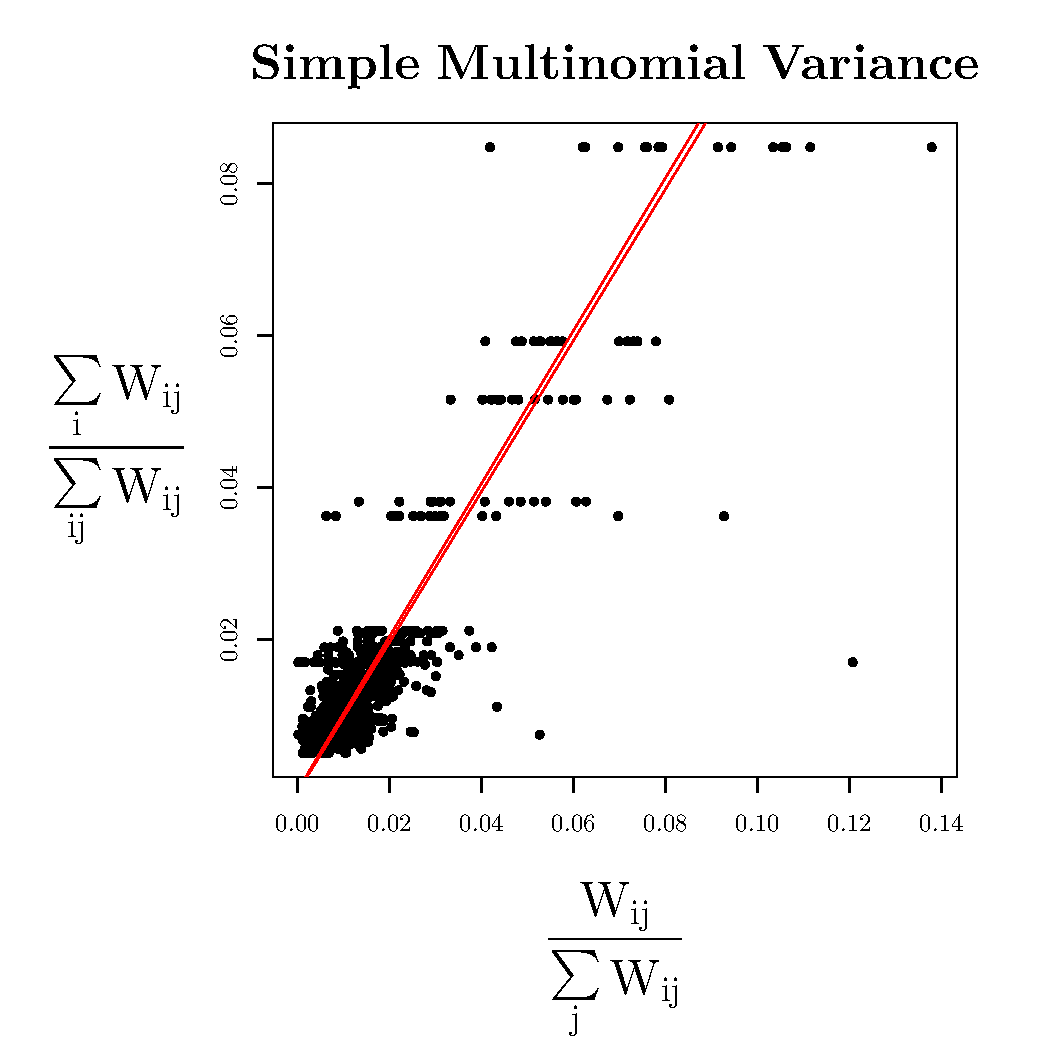
\includegraphics[width=.75\textwidth]{Images/simpleMult11.pdf}
    \caption{These images display the observed composition on the X-axis and the estimated proportions under a simple multinomial model on the Y-axis. The red lines represent the estimated variance of the estimated proportions. Clearly, this model does allow for an appropriate variance model. }\label{fig:simpMult}
\end{figure}



\clearpage

\begin{figure}[ht!]
    \centering
    \begin{subfigure}[b]{0.38\textheight}
        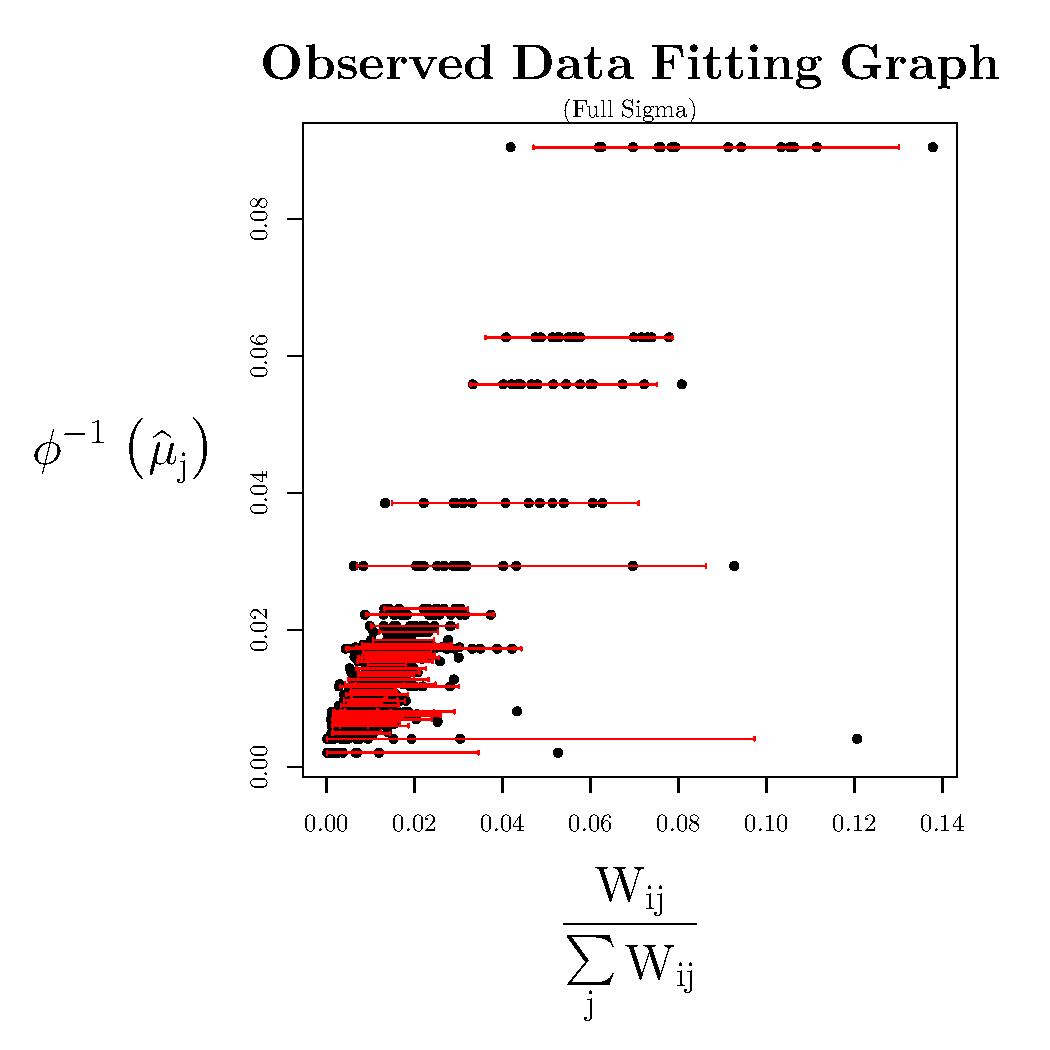
\includegraphics[width=\textwidth]{Images/XiaPlotBars11.pdf}
        \caption{Observed compositional fit vs model estimate.}
        %\label{fig:gull}
    \end{subfigure}
\\
    \begin{subfigure}[b]{0.38\textheight}
        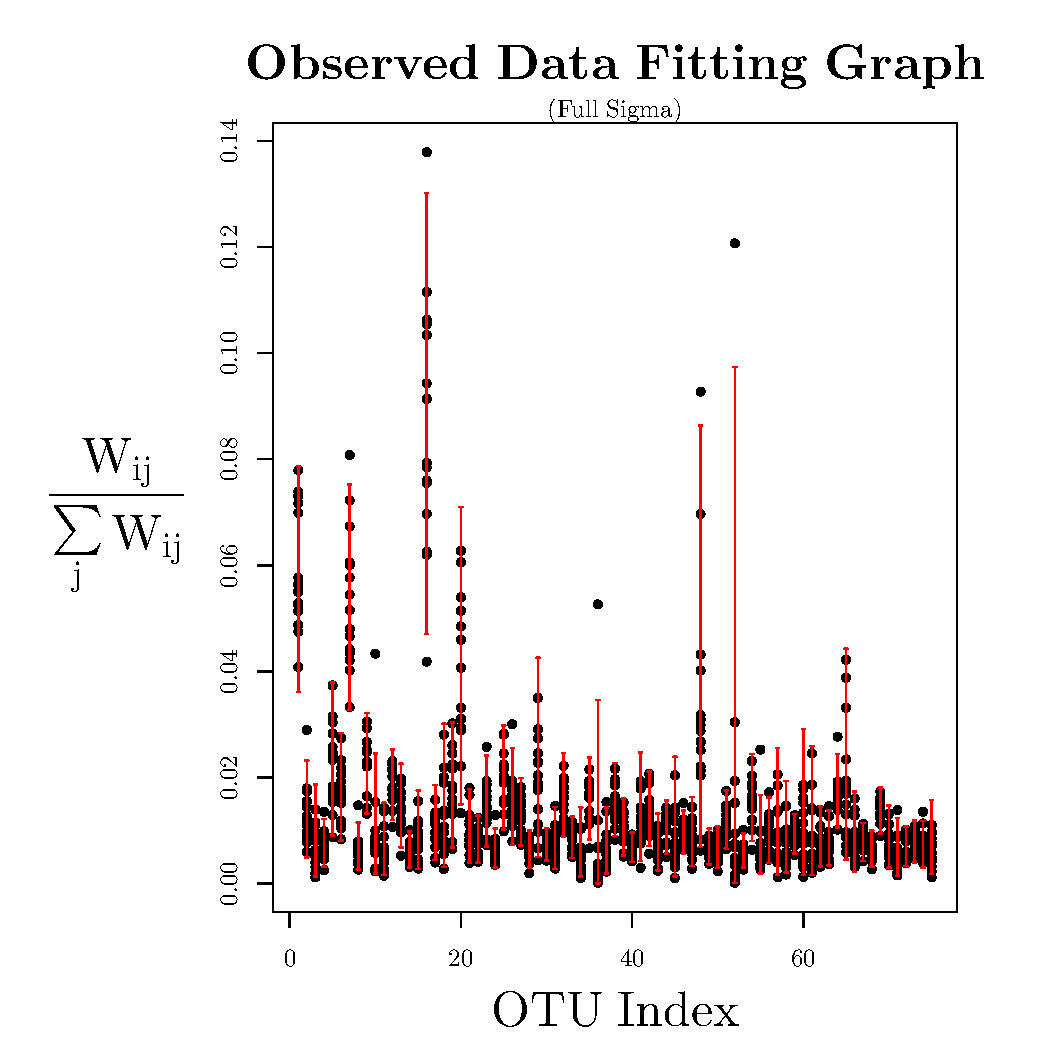
\includegraphics[width=\textwidth]{Images/XiaPlotBars11T.pdf}
        \caption{Observed compositional fit vs model estimate, by OTU.}
        %\label{fig:tiger}
    \end{subfigure}
    \caption{The first image displays the observed composition on the X-axis and $\phi^{-1}(\hat{\mu}_j)$ on the Y-axis. The latter plot separates the data by OTU index. The estimated composition values are constant within columns. The red bars represent the empirical 95\% confidence interval for each estimated composition based on 10,000 simulations from the model fit using the full $\hat{\boldsymbol{\Sigma}}$.}\label{fig:compFitBar}
\end{figure}

\clearpage 

\begin{figure}[ht!]
    \centering
    \begin{subfigure}[b]{0.38\textheight}
        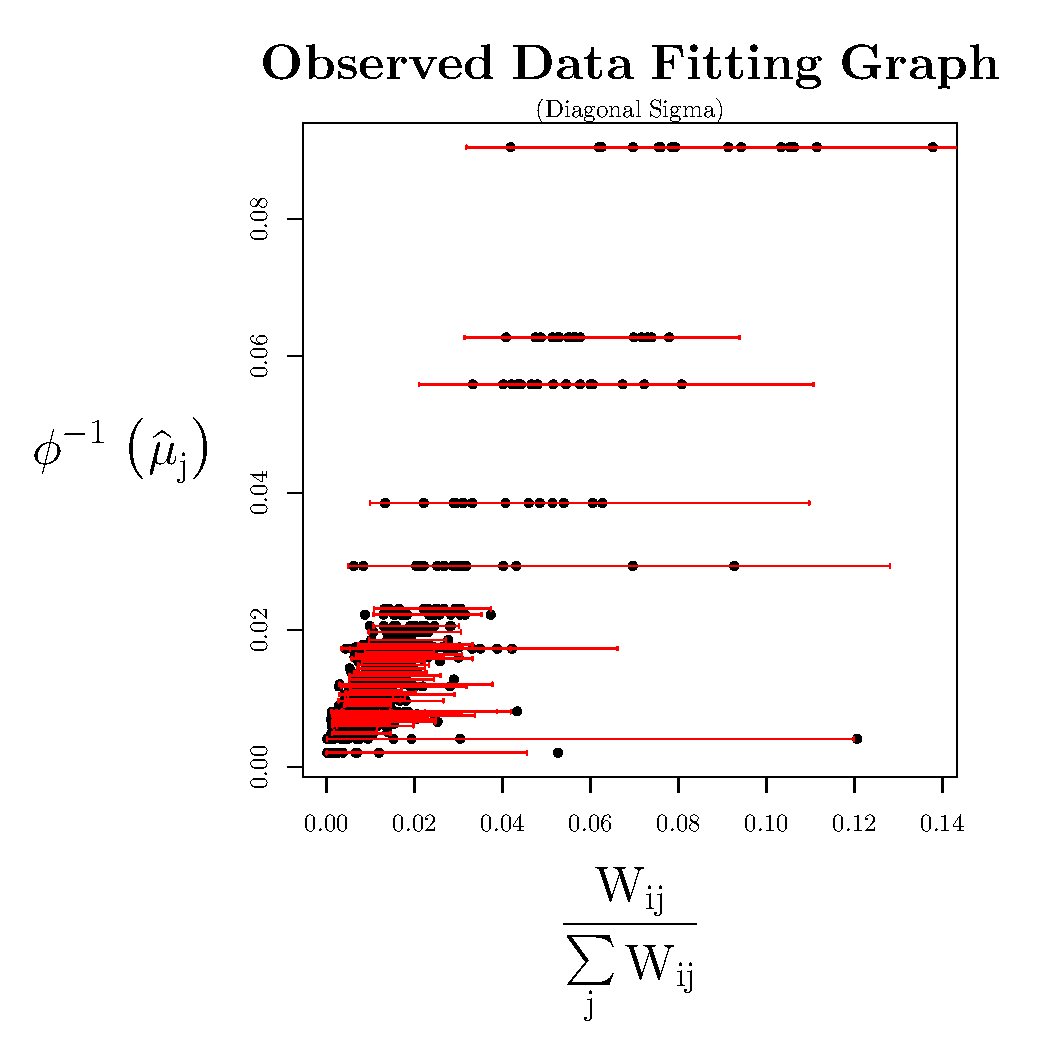
\includegraphics[width=\textwidth]{Images/XiaPlotBars11diag.pdf}
        \caption{Observed compositional fit vs model estimate, using a diagonal covariance.}
        %\label{fig:gull}
    \end{subfigure}
\\
    \begin{subfigure}[b]{0.38\textheight}
        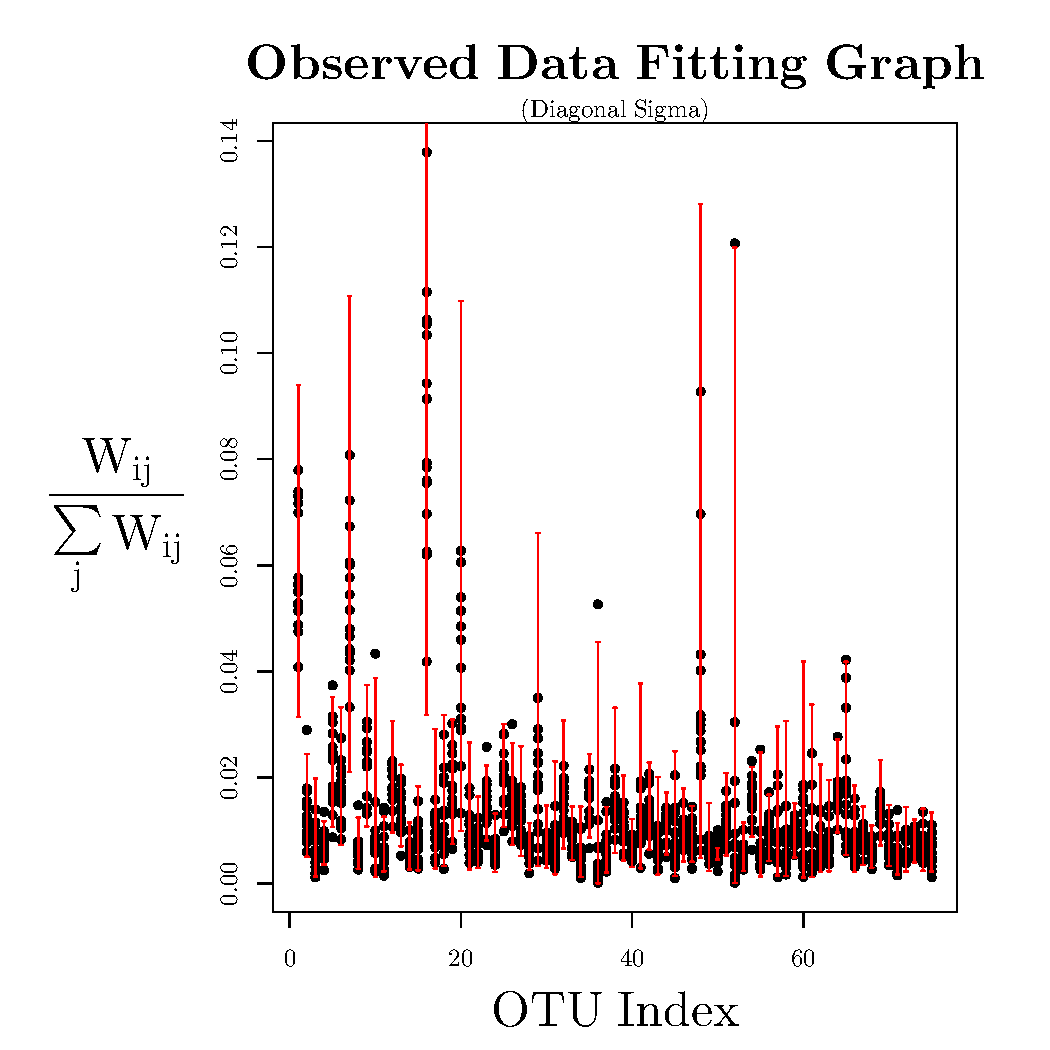
\includegraphics[width=\textwidth]{Images/XiaPlotBars11diagT.pdf}
        \caption{Observed compositional fit vs model estimate, by OTU, using a diagonal covariance.}
        %\label{fig:tiger}
    \end{subfigure}
    \caption{The first image displays the observed composition on the X-axis and $\phi^{-1}(\hat{\mu}_j)$ on the Y-axis. The latter plot separates the data by OTU index. The estimated composition values are constant within columns. The red bars represent the empirical 95\% confidence interval for each estimated composition based on 10,000 simulations from the model fit using only the diagonal of $\hat{\boldsymbol{\Sigma}}$.}\label{fig:compFitBarDiag}
\end{figure}

\clearpage 

\begin{figure}[ht!]
    \centering
    \begin{subfigure}[b]{0.38\textheight}
        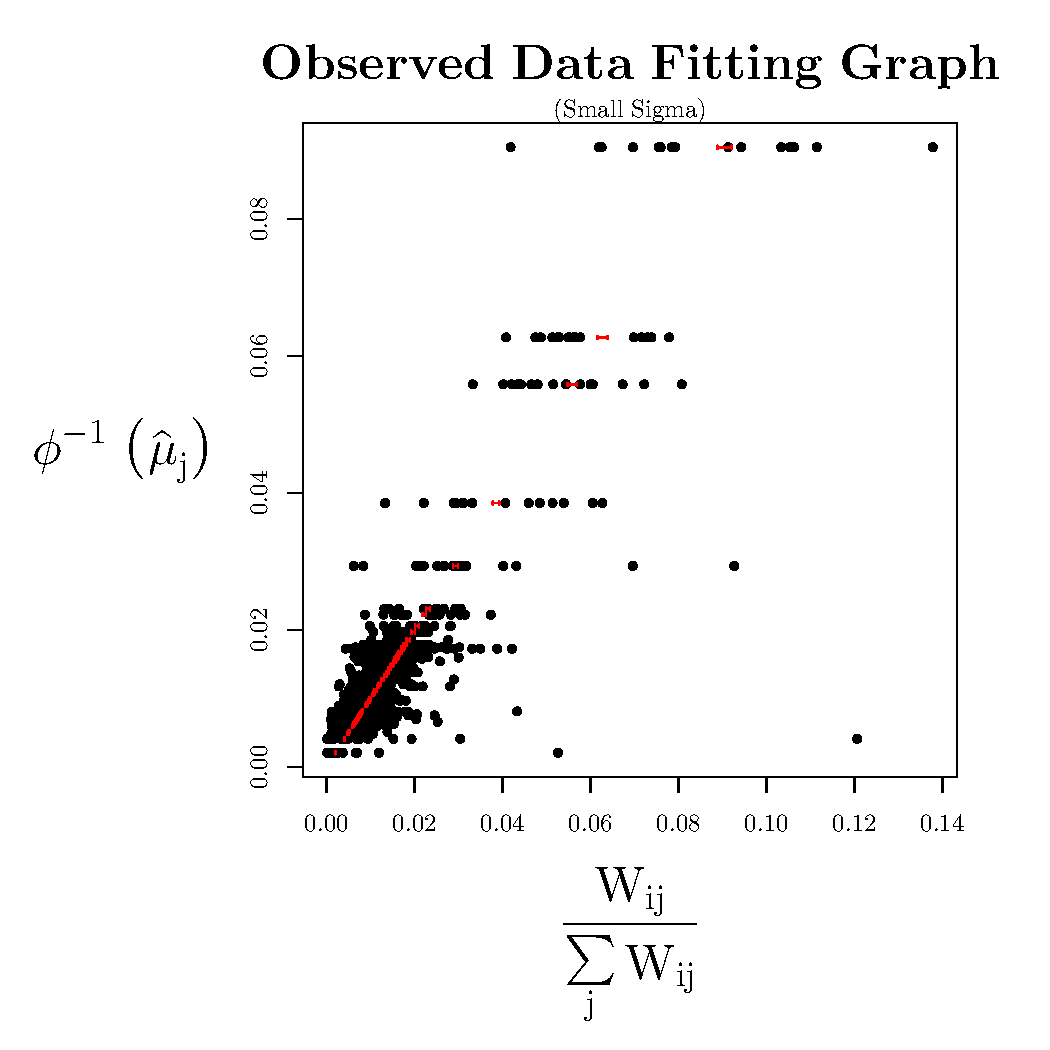
\includegraphics[width=\textwidth]{Images/XiaPlotBars11small.pdf}
        \caption{Observed compositional fit vs model estimate, using a small diagonal covariance.}
        %\label{fig:gull}
    \end{subfigure}
\\
    \begin{subfigure}[b]{0.38\textheight}
        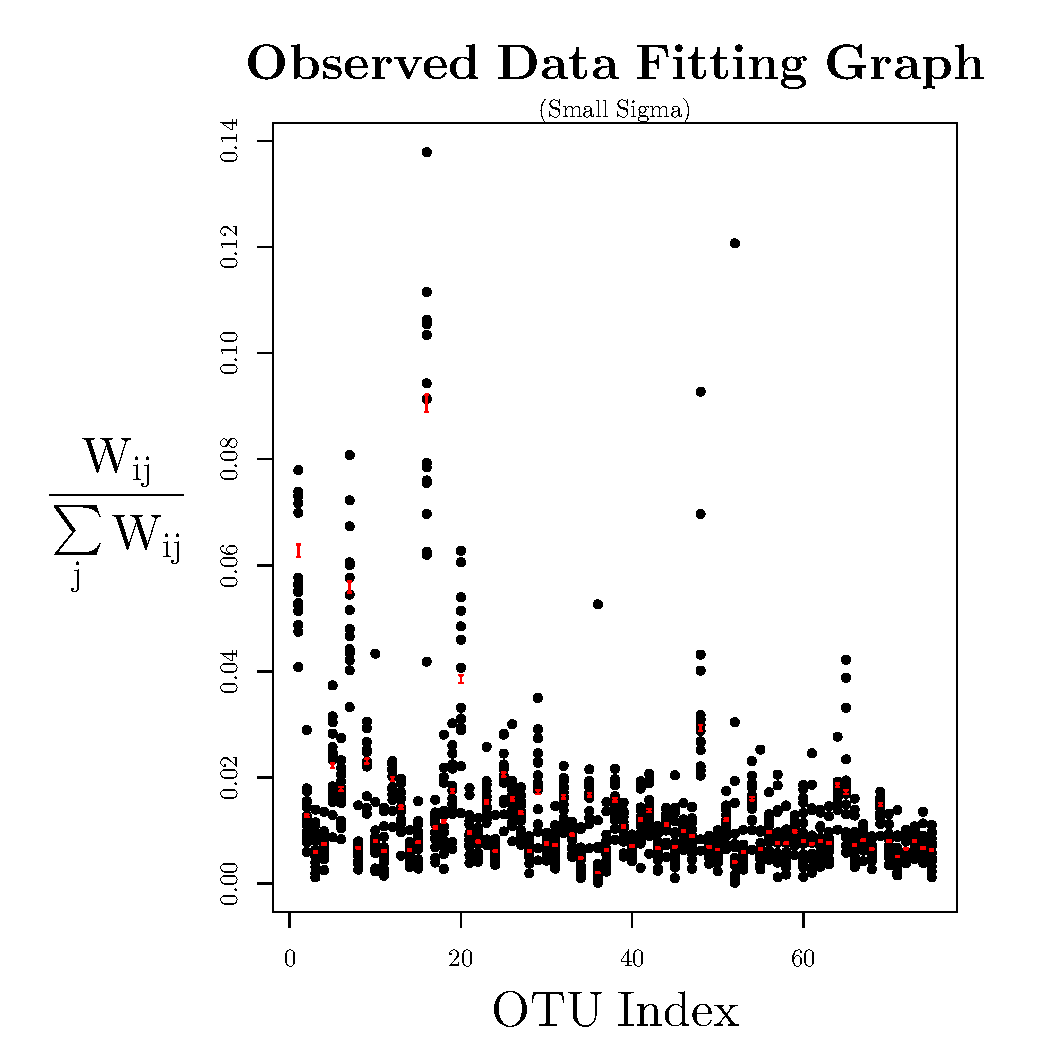
\includegraphics[width=\textwidth]{Images/XiaPlotBars11smallT.pdf}
        \caption{Observed compositional fit vs model estimate, by OTU, using a small diagonal covariance.}
        %\label{fig:tiger}
    \end{subfigure}
    \caption{The first image displays the observed composition on the X-axis and $\phi^{-1}(\hat{\mu}_j)$ on the Y-axis. The latter plot separates the data by OTU index. The estimated composition values are constant within columns. The red bars represent the empirical 95\% confidence interval for each estimated composition based on 10,000 simulations from the model fit using only a diagonal matrix with diagonal values equal to $10^{-5}$ for $\hat{\boldsymbol{\Sigma}}$.}\label{fig:compFitBarSmall}
\end{figure}

\clearpage 

\begin{figure}[ht!]
    \centering
    \begin{subfigure}[b]{0.38\textheight}
        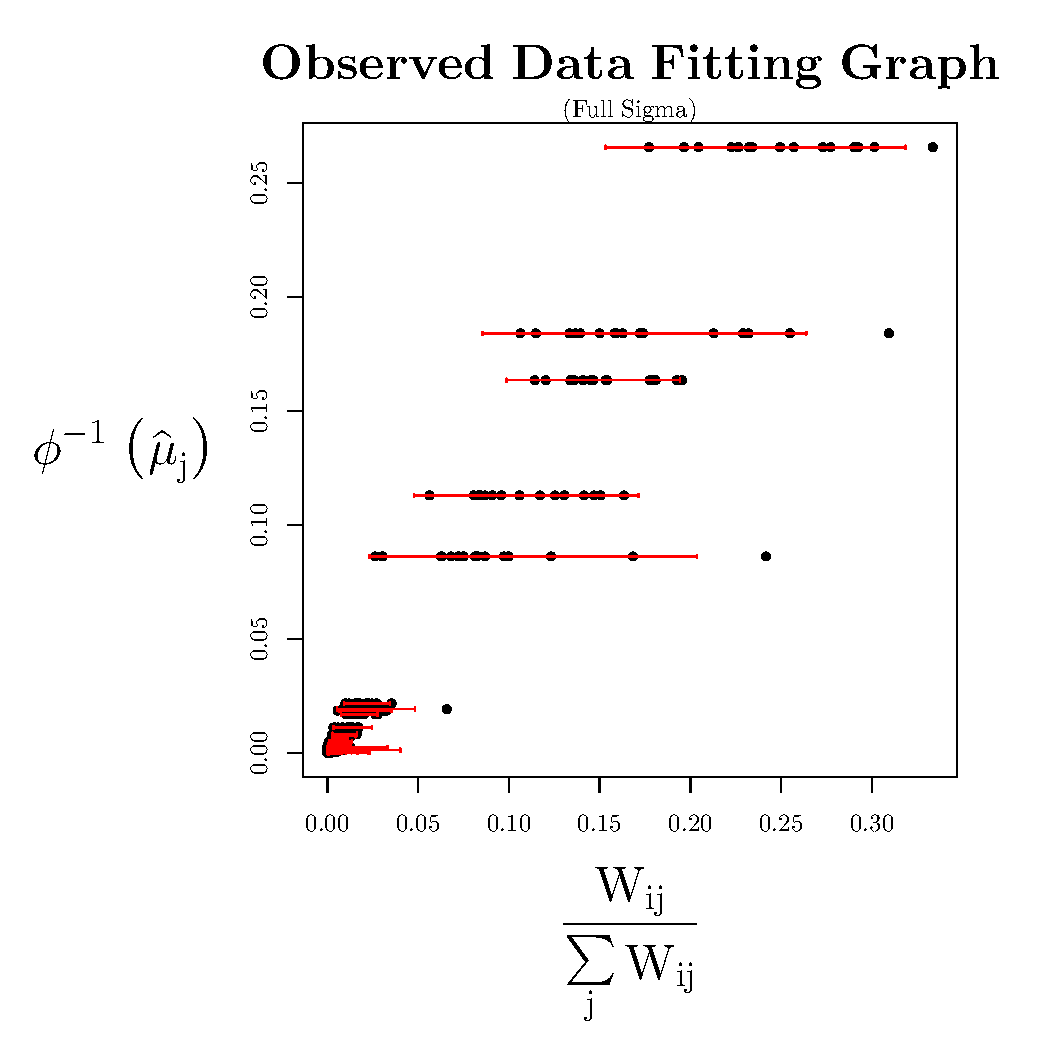
\includegraphics[width=\textwidth]{Images/XiaPlotBars295v5.pdf}
        \caption{Observed compositional fit vs model estimate, using the five most frequent OTUs, and 295 randomly selected OTUs.}
        %\label{fig:gull}
    \end{subfigure}
\\
    \begin{subfigure}[b]{0.34\textheight}
        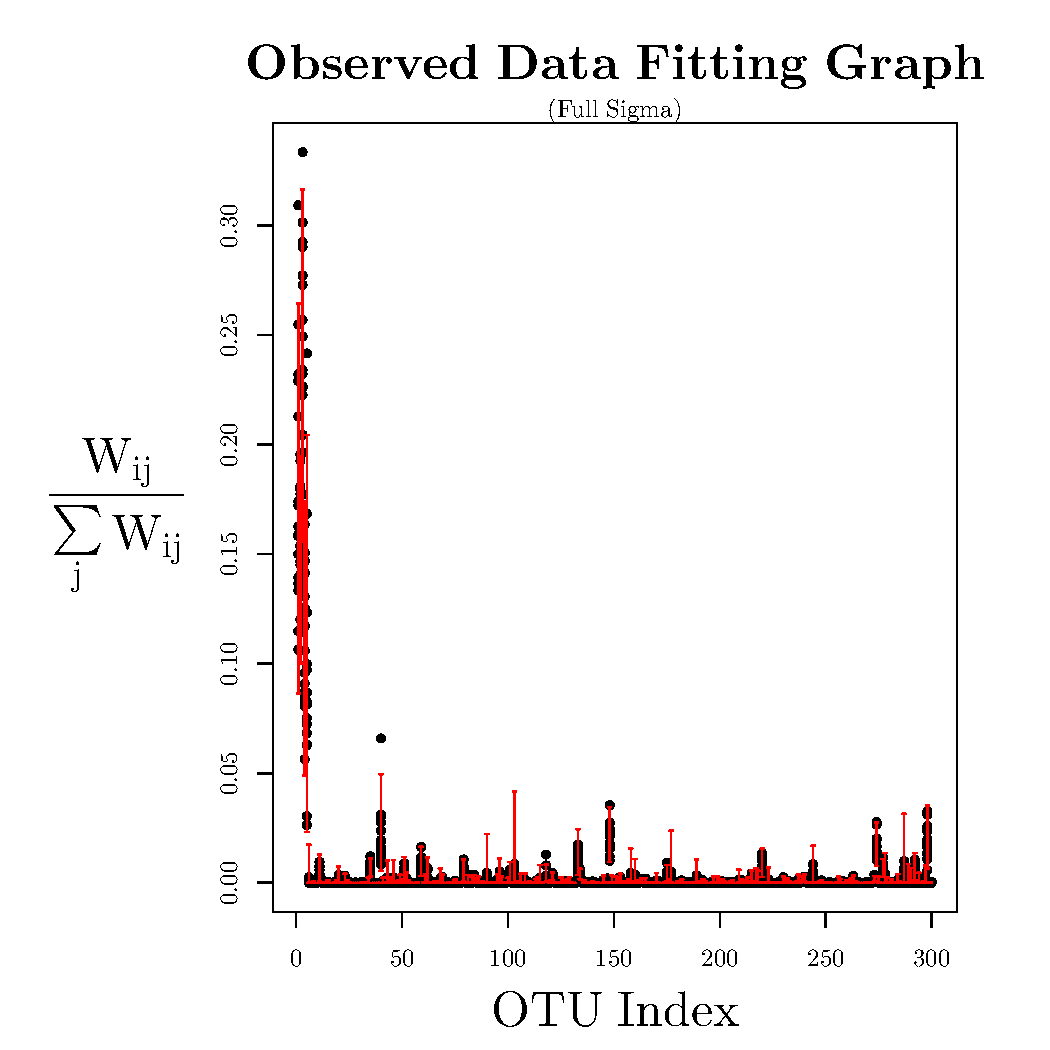
\includegraphics[width=\textwidth]{Images/XiaPlotBars295v5T.pdf}
        \caption{Observed compositional fit vs model estimate, using the five most frequent OTUs, and 295 randomly selected OTUs, by OTU index.}
        %\label{fig:tiger}
    \end{subfigure}
    \caption{The first image displays the observed composition on the X-axis and $\phi^{-1}(\hat{\mu}_j)$ on the Y-axis, with the five most frequent OTUs and 295 randomly selected OTUs. The latter plot separates the data by OTU index. The estimated composition values are constant within columns. The red bars represent the empirical 95\% confidence interval for each estimated composition based on 10,000 simulations from the model fit using $\hat{\boldsymbol{\Sigma}}$.}\label{fig:compFitBar295}
\end{figure}

\clearpage 

\begin{figure}[ht!]
    \centering
    \begin{subfigure}[b]{0.38\textheight}
        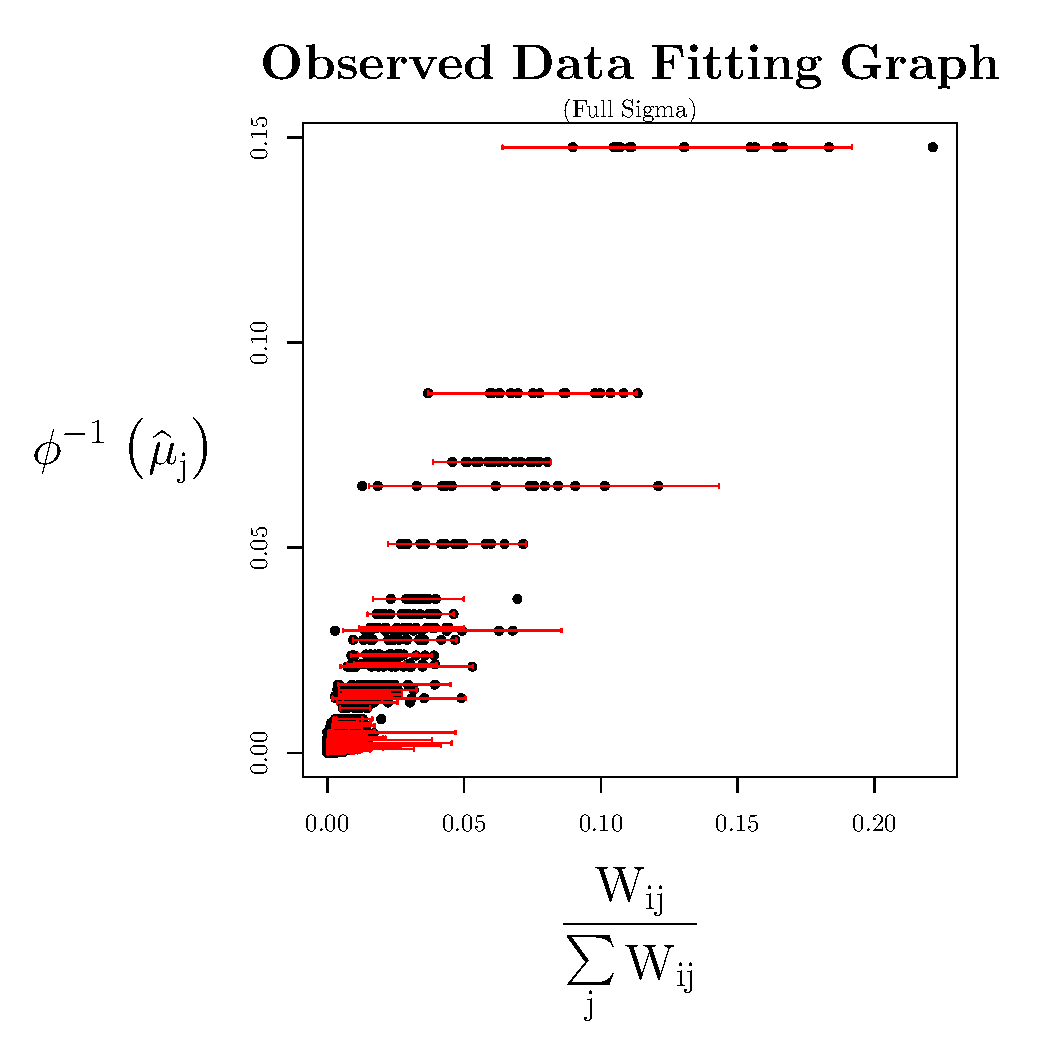
\includegraphics[width=\textwidth]{Images/XiaPlotBars300.pdf}
        \caption{Observed compositional fit vs model estimate, using 300 randomly selected OTUs.}
        %\label{fig:gull}
    \end{subfigure}
\\
    \begin{subfigure}[b]{0.38\textheight}
        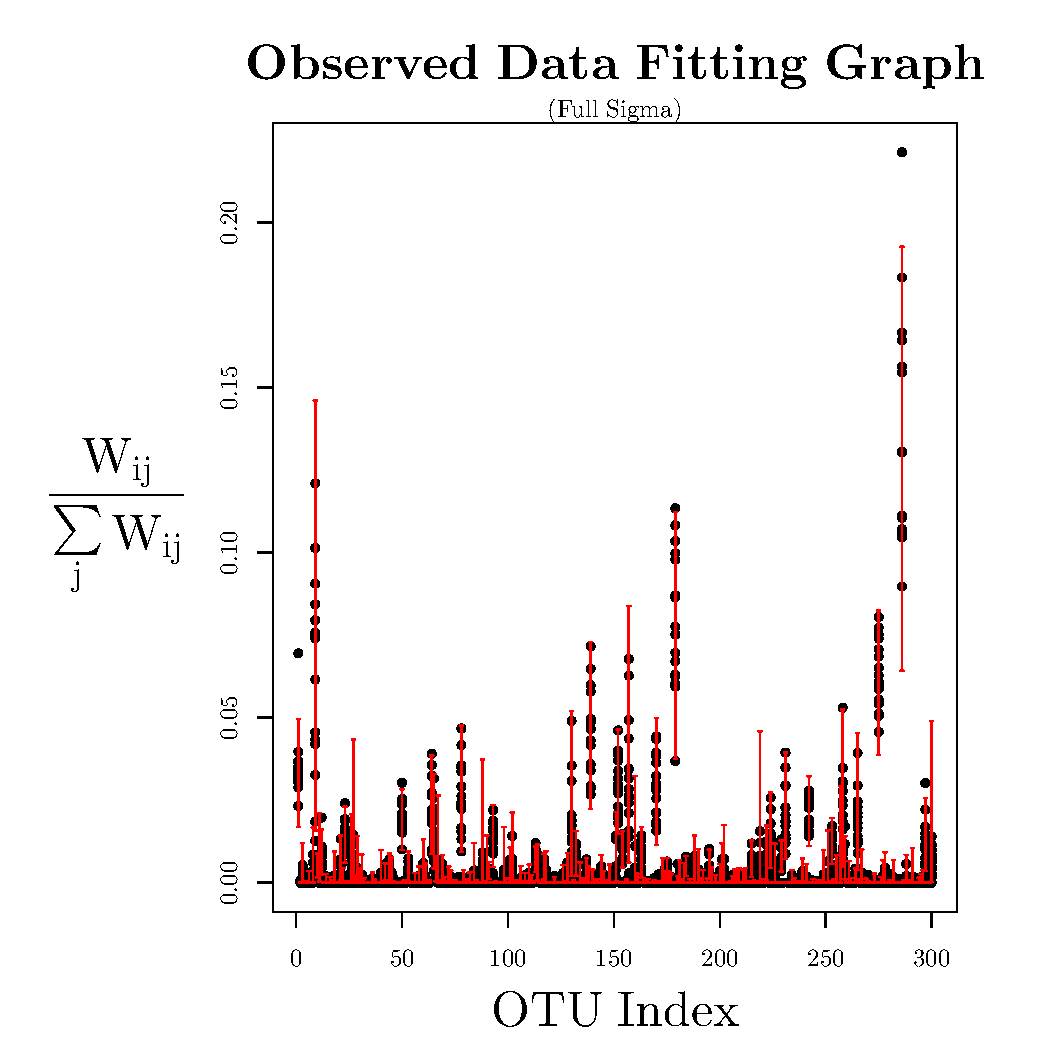
\includegraphics[width=\textwidth]{Images/XiaPlotBars300T.pdf}
        \caption{Observed compositional fit vs model estimate, using 300 randomly selected OTUs, by OTU index.}
        %\label{fig:tiger}
    \end{subfigure}
    \caption{The first image displays the observed composition on the X-axis and $\phi^{-1}(\hat{\mu}_j)$ on the Y-axis, with 300 randomly selected OTUs. The latter plot separates the data by OTU index. The estimated composition values are constant within columns. The red bars represent the empirical 95\% confidence interval for each estimated composition based on 10,000 simulations from the model fit using $\hat{\boldsymbol{\Sigma}}$.}\label{fig:compFitBar300}
\end{figure}


\clearpage 

\begin{figure}[ht!]
    \centering
    \begin{subfigure}[b]{0.36\textheight}
        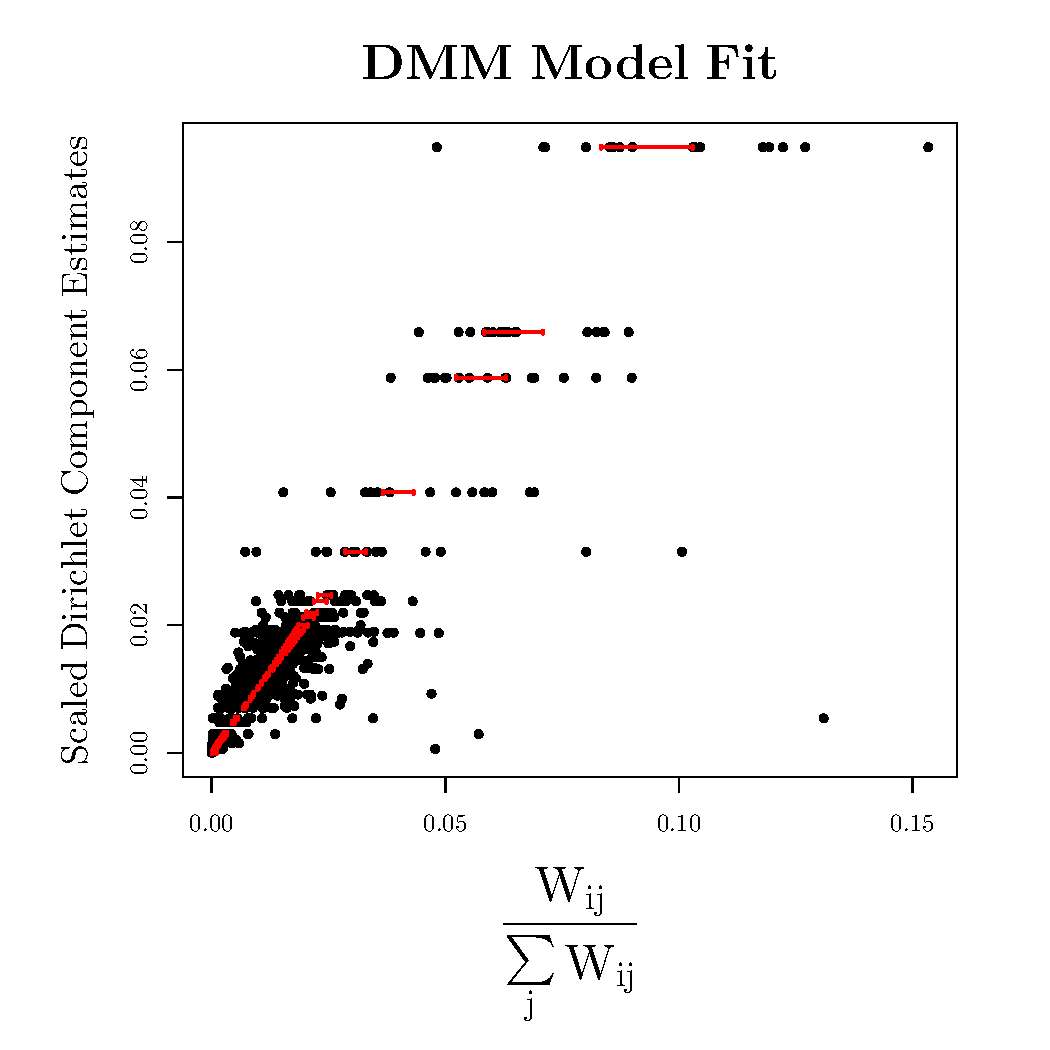
\includegraphics[width=\textwidth]{Images/DMM250.pdf}
        \caption{Observed compositional fit vs model estimate, using the 50 most frequent OTUs and 250 randomly selected OTUs.}
        %\label{fig:gull}
    \end{subfigure}
\\
    \begin{subfigure}[b]{0.36\textheight}
        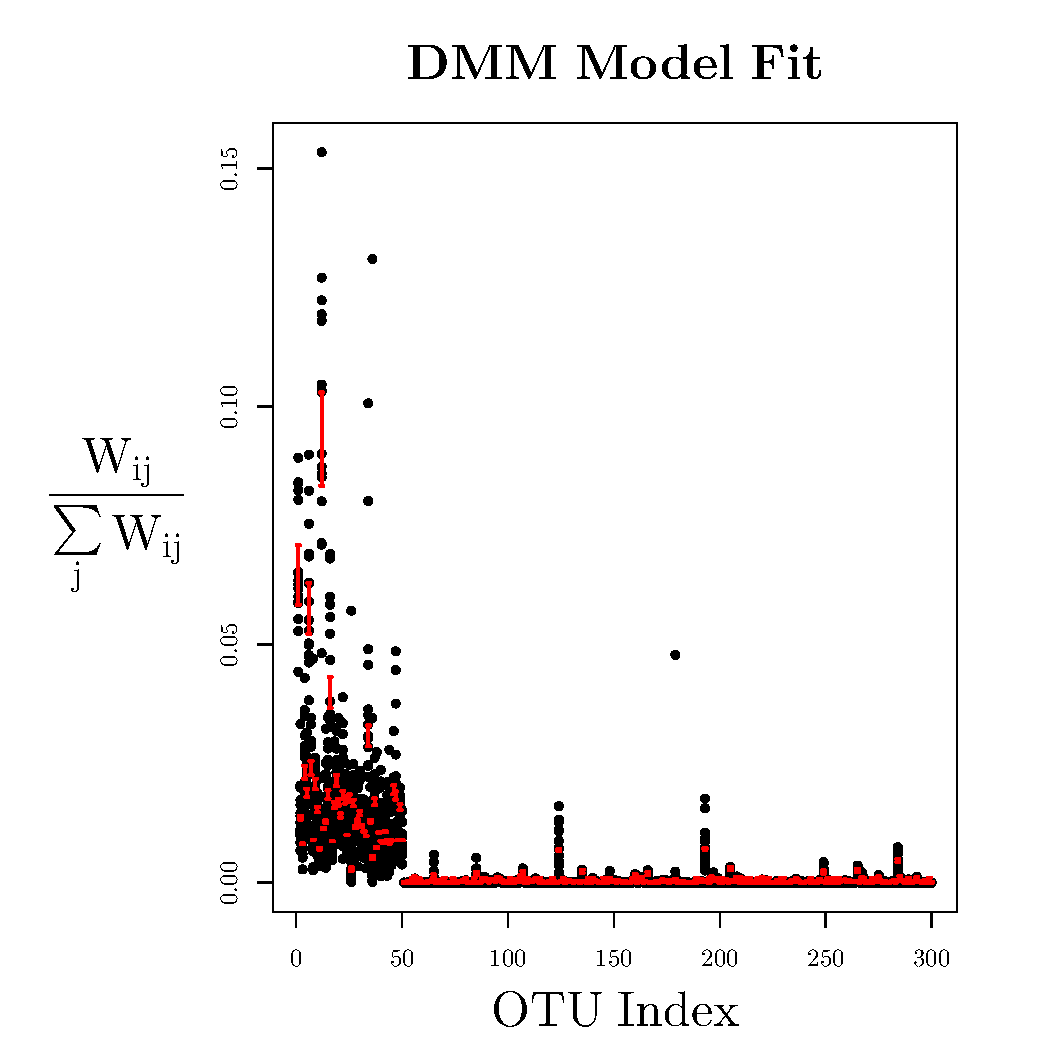
\includegraphics[width=\textwidth]{Images/DMM250T.pdf}
        \caption{Observed compositional fit vs model estimate, the 50 most frequent OTUs and 250 randomly selected OTUs, by OTU index.}
        %\label{fig:tiger}
    \end{subfigure}
    \caption{The first image displays the observed composition on the X-axis and the scaled Dirichlet component estimates on the Y-axis, with the 50 most frequent OTUs and 250 randomly selected OTUs. The latter plot separates the data by OTU index. The estimated composition values are constant within columns. The red bars represent the 95\% confidence interval for each estimated composition.}\label{fig:dmmFitBar250}
\end{figure}

\clearpage 

\begin{figure}[ht!]
    \centering
    \begin{subfigure}[b]{0.36\textheight}
        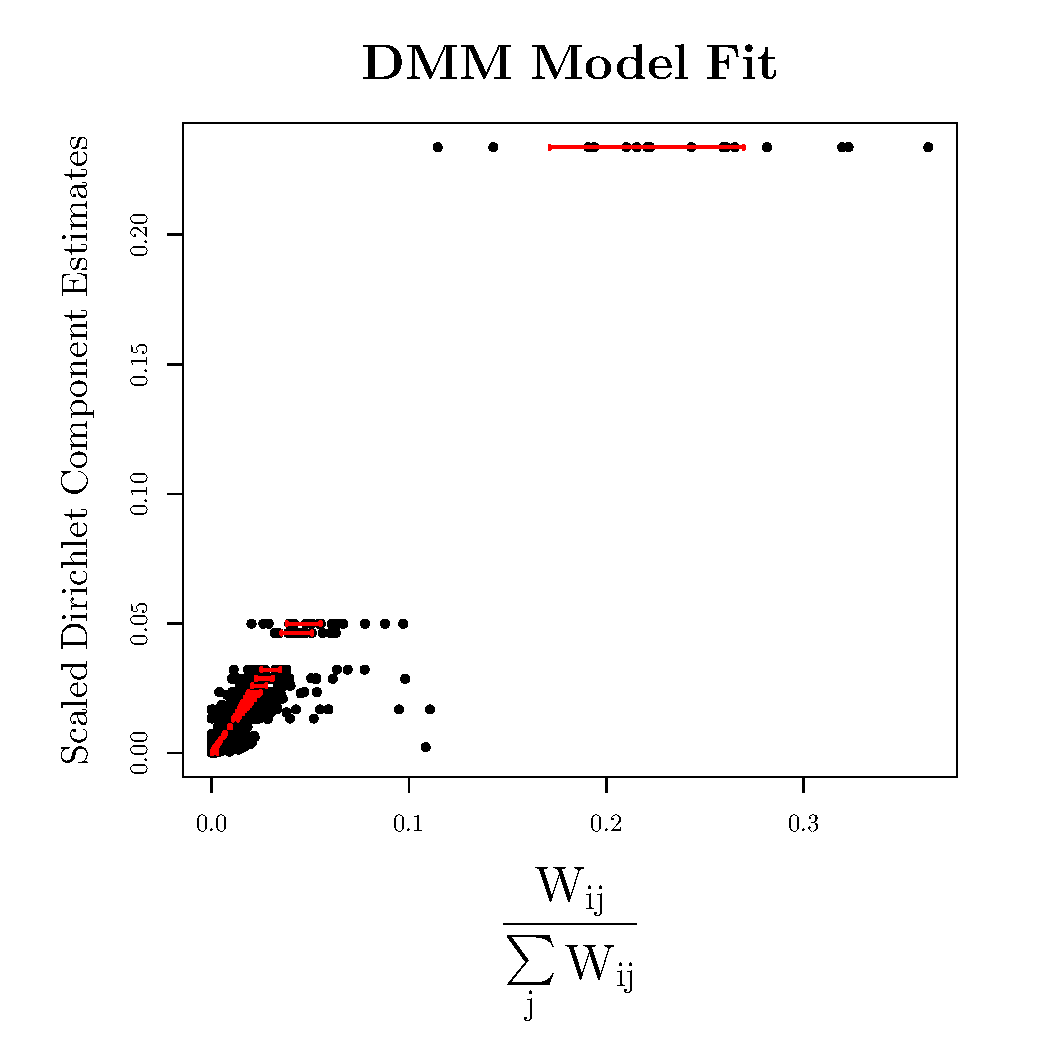
\includegraphics[width=\textwidth]{Images/DMM300.pdf}
        \caption{Observed compositional fit vs model estimate, using 300 randomly selected OTUs.}
        %\label{fig:gull}
    \end{subfigure}
\\
    \begin{subfigure}[b]{0.36\textheight}
        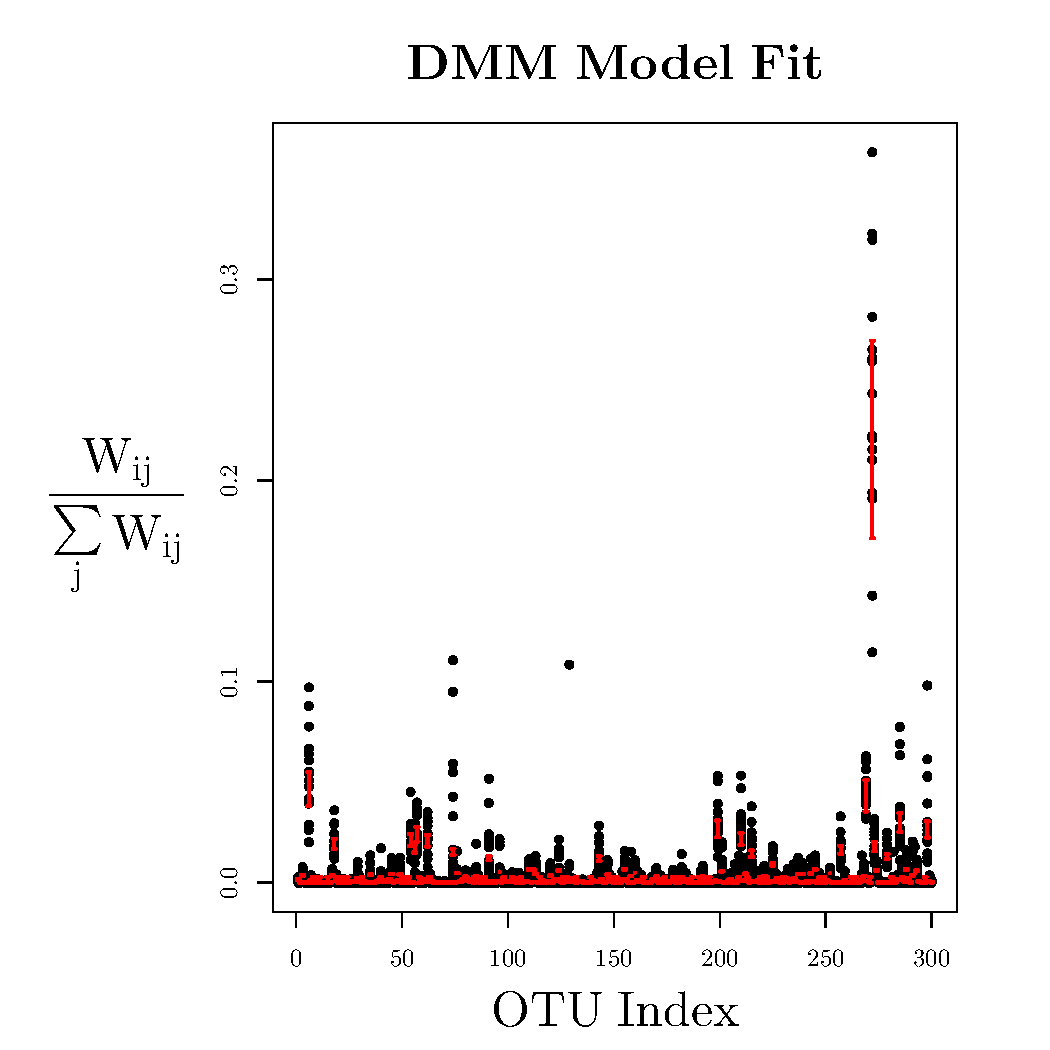
\includegraphics[width=\textwidth]{Images/DMM300T.pdf}
        \caption{Observed compositional fit vs model estimate, the 300 randomly selected OTUs, by OTU index.}
        %\label{fig:tiger}
    \end{subfigure}
    \caption{The first image displays the observed composition on the X-axis and the scaled Dirichlet component estimates on the Y-axis, with 300 randomly selected OTUs. The latter plot separates the data by OTU index. The estimated composition values are constant within columns. The red bars represent the 95\% confidence interval for each estimated composition.}\label{fig:dmmFitBar300}
\end{figure}

\FloatBarrier
\clearpage 


\bibliography{bib}

\end{document}









\begin{comment}
\begin{figure}[ht!]
    \centering
    \begin{subfigure}[b]{0.40\textheight}
        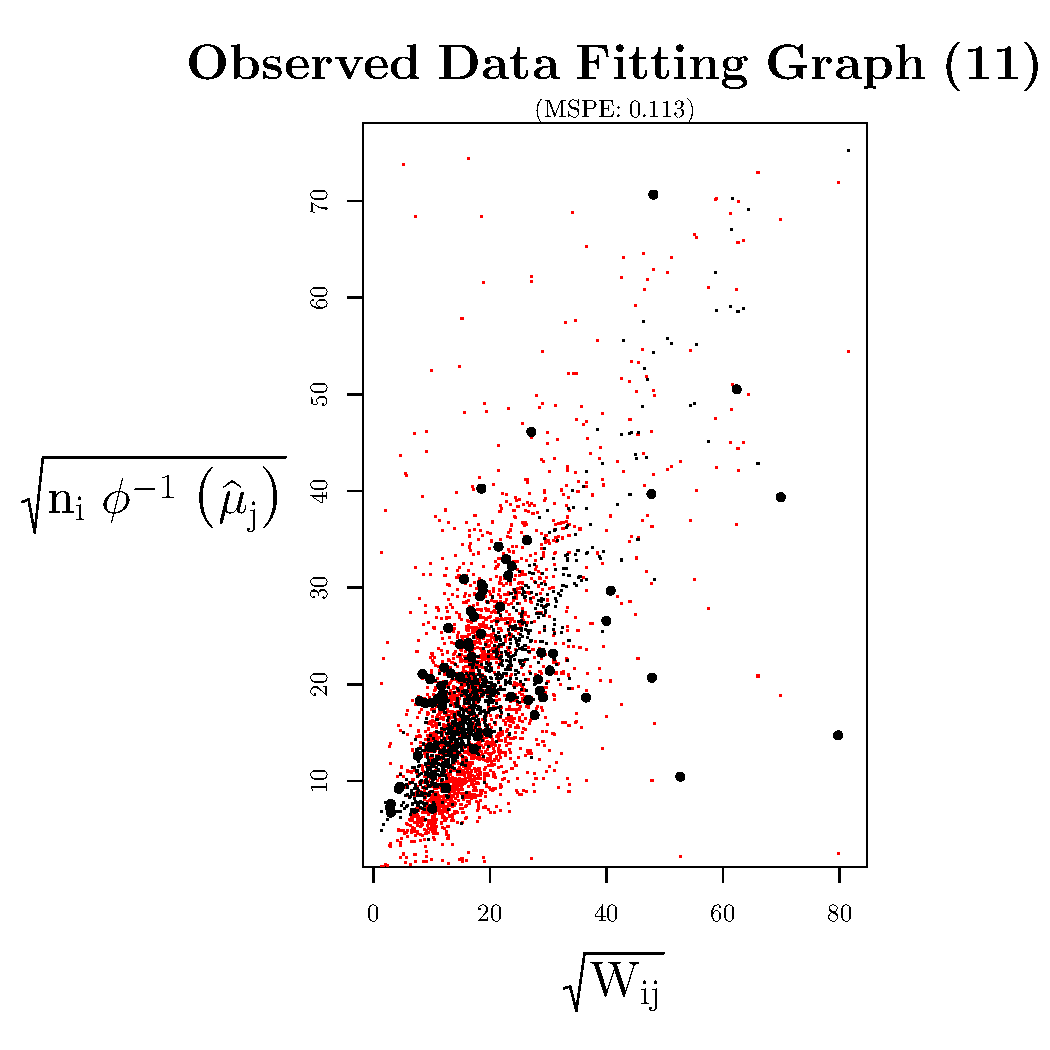
\includegraphics[width=\textwidth]{Images/XiaPlotWBars11.pdf}
        \caption{DayAmdmt = 11}
        %\label{fig:gull}
    \end{subfigure}
\\
    \begin{subfigure}[b]{0.40\textheight}
        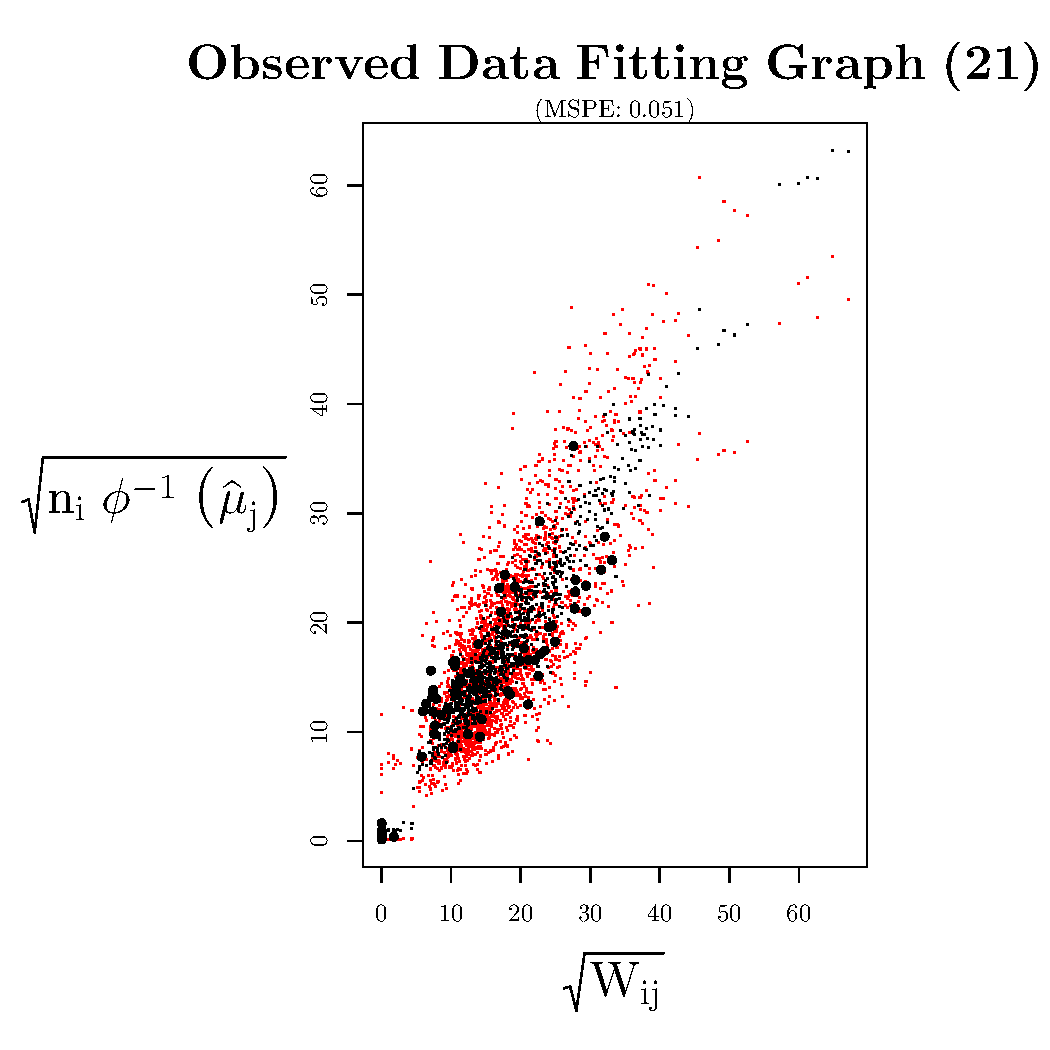
\includegraphics[width=\textwidth]{Images/XiaPlotWBars21.pdf}
        \caption{DayAmdmt = 21}
        %\label{fig:tiger}
    \end{subfigure}
    \caption{These images display the square root of the observed counts $\mbf{W}$ on the X-axis and $\sqrt{n_i\phi^{-1}(\hat{\mu}_j)}$ on the Y-axis. The red dots represent the empirical 95\% confidence interval for each estimated point based on 10,000 simulations from the model fit. The larger points represent observed sample values that were outside of the estimated 95\% confidence interval. }\label{fig:FitBar}
\end{figure}
\end{comment}